\documentclass[12pt]{amsart}    % Specifies the document style.
\usepackage{graphicx, amsfonts, amsmath, amssymb, amsthm, pictexwd,color,ifsym, enumitem, mathrsfs, verbatim} 
\usepackage[cmtip,all,matrix,arrow,tips,curve]{xy}
\usepackage[notref,notcite]{showkeys}
\usepackage[active]{srcltx}
\usepackage[usenames,dvipsnames,svgnames,table]{}

\usepackage{tikz}
%%%< 
\usepackage{verbatim}
%\usepackage[active,tightpage]{preview}
%\PreviewEnvironment{tikzpicture}
\usetikzlibrary{matrix, arrows,decorations.pathmorphing}
%\setlength\PreviewBorder{5pt}%

% The next few lines are formatting commands.
% Do not change them because we
% want all your technical reports to be formatted in a
% similar way.
\textwidth=6.5in
\textheight=9in
\hoffset=-0.75in
\voffset=-0.75in
%\setcounter{page}{19}
\newtheorem{theorem}{Theorem}[section]
\newtheorem{corollary}{Corollary}
\newtheorem{lemma}[theorem]{Lemma}
\newtheorem{proposition}{Proposition}
\theoremstyle{definition}
\newtheorem{example}{Example}
\newtheorem{definition}{Definition}
%%%%%%%%%%%%%%%%%%%%%%%%%%%%%%%%%%%%%%%%%%%%%%%%%%%%%%%%%%%%%%%%
% This is the title information for your report.
% Insert your title in the braces below.
\title{Derived Categories}
% Insert your names (in alpha order) and universities as indicated
\author{Nikki Sanderson, Lucas Simon}
%\date{March 23, 2015}

%%%%%%%%%%%%%%%%%%%%%%%%%%%%%%%%%%%%%%%%%%%%%%%%%%%%%%%%%%%%%%%%
% Do not touch the next two lines
\begin{document}           % End of preamble.
\maketitle                 % Produces the title.
%%%%%%%%%%%%%%%%%%%%%%%%%%%%%%%%%%%%%%%%%%%%%%%%%%%%%%%%%%%%%%%%

\section{Introduction}

We are going to introduce the Derived Category.  

\

We assume knowledge of some vocabulary:

\

\begin{itemize}
\item additive category, additive functor 
\item abelian category
\item k-linear category*
\item category of complexes
\item natural isomorphism
\item null-homotopy
\item quasi-isomorphism
\end{itemize}

\

We'll also need some new tools, which we'll define, explain and motivate:

\

\begin{itemize}
\item triangles (triangulated category)
\item cohomological functors
\item Ore localization
\item right denominator set
\item localization of a triangulated category
\end{itemize}

\

That will be the bulk of the paper.  We will finish with application of the derived category to representations of quivers (?).

\

Our setting is the category of complexes $\textbf{C(M)}$ of an additive category $\textbf{M}$.  We arrive in the homotopy category of complexes $\textbf{K(M)}$ by noting that C(M) is a linear category and the null-homotopic morphisms form a 2-sided ideal, and quotienting by that ideal.  Now is when we mention $\textbf{triangles}$ because K(M) is a $\textbf{triangulated category}$.  It turns out that we get the Derived Category $\textbf{D(M)}$ as the image (?) of a triangulated functor from the homotopy category; as well, it is triangulated.  We construct the Derived Category as the $\textbf{localization}$ of the homotopy category about the quasi-isomorphisms, which are a $\textbf{right denominator set}$.  The key is we can learn about exact sequences in M from distinguished triangles in D(M).

\section{Triangulated Categories}

A $\textbf{T-additive category}$ is an additive category $\textbf{K}$ with an additive automorphsim $\textbf{T}$, called the "translation" or "shift" or "suspension".  A $\textbf{T-additive functor}$ is an additive functor $\textbf{F}: K \rightarrow L$ with a natural isomorphism $\xi: F \circ T_K \rightarrow T_L \circ F$.  It follows that a $\textbf{morphism of T-additive functors}$ is a natural transformation $\eta: (F,\xi) \rightarrow (G, \nu)$ with commutative diagram

\



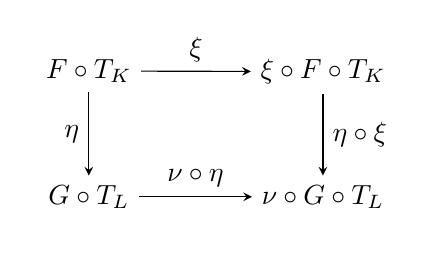
\begin{tikzpicture}
  \matrix (m) [matrix of math nodes,row sep=3em,column sep=4em,minimum width=2em]
  {
     F \circ T_K & \xi \circ F \circ T_K \\
     G \circ T_L & \nu \circ G \circ T_L \\};
  \path[-stealth]
    (m-1-1) edge node [left] {$\eta$} (m-2-1)
            edge node [above] {$\xi $} (m-1-2)
    (m-2-1) edge node [above] {$\nu \circ \eta$} (m-2-2)
    (m-1-2) edge node [right] {$\eta \circ \xi$} (m-2-2);
            
\end{tikzpicture}

\

A $\textbf{triangle}$ is a diagram $L \xrightarrow{\alpha} M \xrightarrow{\beta} N \xrightarrow{\gamma} T(L)$, and a morphism of triangles is a triple of maps $(\phi, \psi, \chi)$ with commutative diagram

\


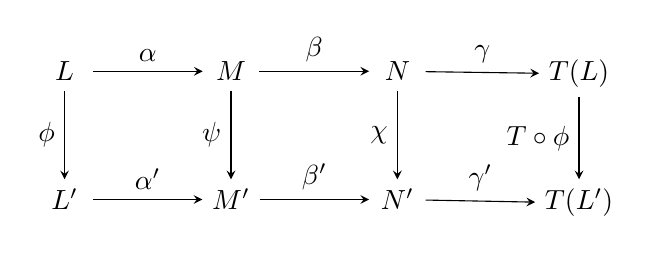
\begin{tikzpicture}
  \matrix (m) [matrix of math nodes,row sep=3em,column sep=4em,minimum width=2em]
  {
     L & M & N & T(L) \\
     L' & M' & N' & T(L') \\};
  \path[-stealth]
    (m-1-1) edge node [left] {$\phi$} (m-2-1)
            edge node [above] {$\alpha $} (m-1-2)
    (m-1-2) edge node [left] {$\psi$} (m-2-2) 
     	      edge node [above] {$\beta$} (m-1-3)
    (m-1-3) edge node [above ] {$\gamma$} (m-1-4)
                edge node [left] {$\chi$} (m-2-3)	  
    (m-1-4) edge node [left] {$ T \circ \phi$} (m-2-4)                     
    (m-2-1) edge node [above] {$\alpha'$} (m-2-2)
    (m-2-2) edge node [above] {$\beta'$} (m-2-3)
    (m-2-3) edge node [above] {$\gamma'$} (m-2-4);     
\end{tikzpicture}



A $\textbf{triangulated category}$ is a T-additive category with a set of $\textbf{distinguished triangles*}$, and a $\textbf{triangulated functor}$ is a T-additive functor that sends distinguished triangles to distinguished triangles.

\

A set of distinguished triangles must satisfy the following axioms:

\

(TR1) If $A$ is isomorphic to $B$ and $B$ is a distinguished triangle, so is $A$.  For every $\alpha: L \rightarrow M$, there is a distinguished triangle $L \xrightarrow{\alpha} M \rightarrow N \rightarrow T(L)$.  For every $M \in K$, $M \xrightarrow{1_M} M \rightarrow 0 \rightarrow T(M)$ is distinguished.

\

(TR2) The triangle $L \xrightarrow{\alpha} M \xrightarrow{\beta} N \xrightarrow{\gamma} T(L)$ is distinguished if and only if $M \xrightarrow{\beta} N \xrightarrow{\gamma} T(L) \xrightarrow{-T(\alpha)} T(M)$ is distinguished.

\

(TR3) If $L \xrightarrow{\alpha} M \xrightarrow{\beta} N \xrightarrow{\gamma} T(L)$ and $L' \xrightarrow{\alpha'} M' \xrightarrow{\beta'} N' \xrightarrow{\gamma'} T(L')$ are distinguished triangles and $\phi: L \rightarrow L', \psi: M \rightarrow M'$ are such that $\psi \circ \alpha = \alpha' \circ \phi$, there exists a $\chi: N \rightarrow N'$ such that we get a morphism of triangles.  

\

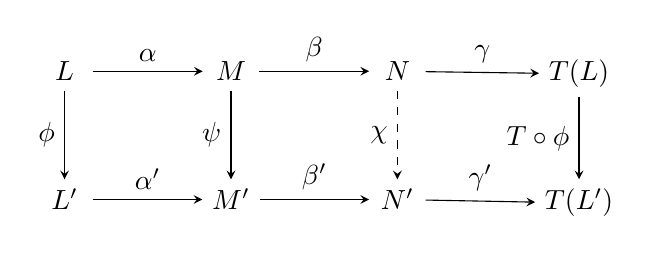
\begin{tikzpicture}
  \matrix (m) [matrix of math nodes,row sep=3em,column sep=4em,minimum width=2em]
  {
     L & M & N & T(L) \\
     L' & M' & N' & T(L') \\};
  \path[-stealth]
    (m-1-1) edge node [left] {$\phi$} (m-2-1)
            edge node [above] {$\alpha $} (m-1-2)
    (m-1-2) edge node [left] {$\psi$} (m-2-2) 
     	      edge node [above] {$\beta$} (m-1-3)
    (m-1-3) edge node [above ] {$\gamma$} (m-1-4)
                edge [dashed]   node [left] {$\chi$} (m-2-3)	  
    (m-1-4) edge node [left] {$ T \circ \phi$} (m-2-4)                     
    (m-2-1) edge node [above] {$\alpha'$} (m-2-2)
    (m-2-2) edge node [above] {$\beta'$} (m-2-3)
    (m-2-3) edge node [above] {$\gamma'$} (m-2-4);     
\end{tikzpicture}

\

(TR4) If $L \xrightarrow{\alpha} M \xrightarrow{\beta} N' \rightarrow T(L), M \xrightarrow{\gamma} N \xrightarrow{\lambda} L' \rightarrow T(M)$ and $L \xrightarrow{\gamma \circ \alpha} N \xrightarrow{\epsilon} M' \rightarrow T(L)$ are distinguished triangles, there exists a distinguished triangle $N' \xrightarrow{\phi} M' \xrightarrow{\psi} L' \rightarrow T(N')$ such that the following diagram commutes

\

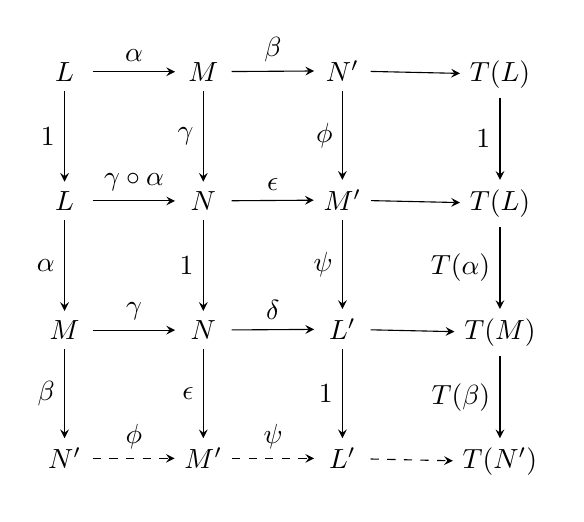
\begin{tikzpicture}
  \matrix (m) [matrix of math nodes,row sep=3em,column sep=3em,minimum width=2em]
  {
     L & M & N' & T(L) \\
     L & N & M' & T(L) \\
     M & N & L' & T(M) \\
     N' & M' & L' & T(N') \\};
  \path[-stealth]
    (m-1-1) edge node [left] {1} (m-2-1)
            edge node [above] {$\alpha$} (m-1-2)
    (m-1-2) edge node [left] {$\gamma$} (m-2-2) 
     	      edge node [above] {$\beta$} (m-1-3)
    (m-1-3) edge (m-1-4)
                edge node [left] {$\phi$} (m-2-3)	  
    (m-1-4) edge node [left] {1} (m-2-4)                     
    (m-2-1) edge node [above] {$\gamma \circ \alpha$} (m-2-2)
    		edge node [left] {$\alpha$} (m-3-1)
    (m-2-2) edge node [above] {$\epsilon$} (m-2-3)
    		edge node [left] {1} (m-3-2)
    (m-2-3) edge (m-2-4) 
    		edge node [left] {$\psi$} (m-3-3)
   (m-2-4) edge node [left] {$T(\alpha)$} (m-3-4)
   (m-3-1) edge node [above] {$\gamma$} (m-3-2)
   		edge node [left] {$\beta$} (m-4-1)
  (m-3-2) edge node [above] {$\delta$} (m-3-3)
  		edge node [left] {$\epsilon$} (m-4-2)
  (m-3-3) edge node [left] {1} (m-4-3)
  		edge (m-3-4)
 (m-3-4) edge node [left] {$T(\beta)$} (m-4-4)
 (m-4-1) edge [dashed] node [above] {$\phi$} (m-4-2)
 (m-4-2) edge [dashed] node [above] {$\psi$} (m-4-3)
 (m-4-3) edge [dashed] (m-4-4);
\end{tikzpicture}


\

- - - EXPLAINATION AND MOTIVATION OF TRIANGLE AXIOMS ; ***BIG IMPORTANT NOTE on 3: NOT FUNCTORIAL, DEEP CONSEQUENCES!!!***
- - - - -

\

\subsection{Getting K(M) is a triangulated category}

\

We begin by defining the standard triangle associated to $\alpha$ when $\alpha: L \rightarrow M$ is a morphism of chain complexes in C(M).  Let $N[i] = L[i+1]\oplus M[i]$ and define the boundary operator $d_N^i: N^i \rightarrow N^{i+1} = $ 

\

INSERT ARRAY

\

.  We call $\textbf{N}$ the $\textbf{mapping cone}$ of $\alpha$ and denote it by cone($\alpha$).  Let $\beta: M \rightarrow N$ be given by 

\

INSERT ARRAY

\

 and $\gamma: N \rightarrow L[1]$ be given by 
 
 \
 
 INSERT ARRAY
 
 \
 
 .  We get a triangle $L \xrightarrow{\alpha} M \xrightarrow{\beta} N \xrightarrow{\gamma} L[1]$. Passing to K(M), we get the $\textbf{standard triangle}$ associated to $\alpha$ $L \xrightarrow{\overline{\alpha}} M \xrightarrow{\overline{\beta}} N \xrightarrow{\overline{\gamma}} L[1]$.  The category K(M) becomes a triangulated category with set of distinguished triangles those isomorphic in K(M) to standard triangles in K(M).  

\

One should now check that this set of distinguished triangles satisfies the necessary axioms (T1), (T2), (T3), (T4).

\

\section{Cohomological Functors (tangent, aside? understand use better):}

\

Now that we have triangulated categories, we can talk about special additive functors from triangulated categories to abelian categories.  A $\textbf{cohomological functor}$ is an additive functor $F: K \rightarrow M$ from a triangulated category to an abelian category such that every distinguished triangle $L \xrightarrow{\alpha} M \xrightarrow{\beta} N \xrightarrow{\gamma} T(L)$ in $K$ gets mapped to an exact sequence $F(L) \xrightarrow{F(\alpha)} F(M) \xrightarrow{F(\beta)} F(N)$. 

\

Two propositions that are nice (? WHY):
\

1) $F: K \rightarrow M$ cohomological, $L \xrightarrow {\alpha} M \xrightarrow{\beta} N \xrightarrow{\gamma} T(L)$ distinguished in K.  Then get LES $ \hdots \rightarrow F(L[i]) \xrightarrow{F(\alpha[i])} F(M[i]) \xrightarrow{F(\beta[i[)} F(N[i]) \xrightarrow{F(\gamma[i])} F(L[i+1]) \xrightarrow{F(\alpha[i+1])} F(M[i+1]) \rightarrow \hdots$.

\

2) K, triangulated. $L \xrightarrow{\alpha} M \xrightarrow{\beta} N \xrightarrow{\gamma} T(L)$, distinguished.  Then $\beta \circ \alpha = 0$. Also for $P \in Ob(K)$, Hom( -, P): $K^{op} \rightarrow$ Ab and Hom(P,-): $K \rightarrow $Ab are cohomological.

\

EXPLAIN AND MOTIVATE. 

\section{Localization}


A $\textbf{weak localization of A with respect to S}$ is a pair $\textbf{(A$_S$, Q)}$ consisting of a category $A_S$ and a functor $Q: A \rightarrow A_S$ such that (i) for all $s \in S, Q(s) \in A_S$ is invertible and (ii) if $F: A \rightarrow B$ is a functor such that $F(s)$ is an isomorphism for $s \in S$, there exists a pair $(F_S, \eta)$ with $F_S: A_S \rightarrow B$ and $\eta: F \rightarrow F_S \circ Q$ an isomorphism of functors.  The pair $(F_s, \eta)$ is unique up to unique isomorphism and the pair $(A_s, Q)$ is unique up to unique equivalence (? CHECK, AND UNDERSTAND IMPORTANCE).

\

A $\textbf{strict localization of A with respect to S}$ is a pair $(A_S, Q)$ such that (i) for all $s \in S, Q(s) \in A_S$ is invertible, (ii) Ob(A$_S$) = Ob(A) and Q is the identity on objects, and (iii) if $F: A \rightarrow B$ is such that $F(s)$ is invertible for all $s \in S$, then there exists $F_S: A_S \rightarrow B$ with $F_S \circ Q = F$ as functors. The pair $(A_S,Q)$ is unique up to unique isomorphism of categories.  (? UNDERSTAND DIFFERENCE W WEAK, EXPLAIN CONNECTION.)

\

A $\textbf{right Ore localization of A with respect to S}$ is a pair $(A_S, Q)$ satisfying 

\

(L1) Ob(A$_S$) = Ob(A), Q identity on objects

\

(L2) for all $s \in S, Q(s) \in A_S$ invertible

\

(L3) for all $q \in A_S$, there exists an $a \in A$ and an $s \in S$ such that $q = Q(a) \circ Q(s)^{-1}$

\

(L4) for all $a, b \in A$ such that $Q(a) = Q(b)$, there exists an $s \in S$ such that $a \circ s = b \circ s$

\

CONNECT TO PREVIOUS WEAK/STRICT, mention left/right, AND TO NEXT RIGHT DENOMINATOR SET.

\

A $\textbf{right denominator set}$ is a multiplicatively closed subset satisfying

\

(D1) (Right Ore condition) for all $a \in A, s \in S$, there exist  $b \in A, t \in S$ such that $a \circ t = s \circ b$

\

(D2) (Right cancellation condition) for all $a, b \in A, s \in S$ s.t. $s \circ a = s \circ b$, there exists a $t \in S$ such that $a \circ t = b \circ t$

\

*DIAGRAMS* OF THESE CONDITIONS


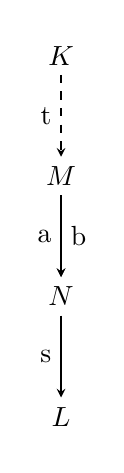
\begin{tikzpicture}
\matrix (m) [matrix of math nodes, row sep=3em, column sep=3em]{
K \\
M \\
N \\
L\\};
\path[-stealth]
(m-1-1) edge [dashed] node [left] {t} (m-2-1)
(m-2-1) edge node [left] {a} (m-3-1) edge node [right] {b} (m-3-1)
(m-3-1) edge node [left] {s} (m-4-1);
\end{tikzpicture}

\begin{tikzpicture}
  \matrix (m) [matrix of math nodes, row sep=3em,
    column sep=3em]{
    & K  & \\
    M & & N \\
    & L &\\};
  \path[-stealth]
    (m-1-2) edge [dashed] node [left] {t} (m-2-1) 
    		edge [dashed] node [right] {b} (m-2-3)
    (m-2-1) edge node [left] {a} (m-3-2)
    (m-2-3) edge node [right] {s} (m-3-2);
            \end{tikzpicture}

\

SOME STORY AND EXPLANATIONS OF CONNECTING PROOF PIECES, TIE TOGETHER ORE AND DENOMINATOR SET, ROOFS, EQUIVALENCES; 


\

Let $A$ be a category and $M, N \in Ob(A)$ and consider $A(M,N) = Hom_A(M,N)$.  A $\textbf{multiplicatively closed set S in A}$ is a subset $S(M,N) \subset A(M,N)$ that contains $1_M \in S(M,M)$ and for all $s \in S(L,M), t \in S(M,N)$ we have $t \circ s \in S(L,N)$.  

\

IMPORTANT THEOREM (b/c it comes with a prooof!): 10.2.6: For $S \subset A$ a multiplicatively closed subset, right Ore localization $(A_S, Q)$ exists $\iff$ S is a right denominator set.  

\

% BIG PROOF. INCLUDE. (this is where well-defined based on choice of representative comes in) (this IS where we use Lemma 10.2.7, right Ore condition implies $\sim$ is an equivalence - use to define set A$_S$)

\

\begin{proof}

We begin with proving that the existence of the right Ore localization $(A_S, Q)$ implies that S is a right denominator set; this is the easy/shorter direction (rather, it doesn't involve roofs!).  First we'll show (D1) is satisfied.  Take $a \in A, s \in S$ and consider $q = Q(s)^{-1}\circ Q(a)$.  By (L3) there exists a $b \in A$ and $t \in S$ such that $q = Q(b) \circ Q(t)^{-1}$.  Since $Q(s)^{-1}\circ Q(a) = Q(b) \circ Q(t)^{-1}$, we get $Q(s) \circ Q(b) = Q(a) \circ Q(t)$ so $Q(s \circ b) = Q(a \circ t)$.  By (L4), there exists a $u \in S$ such that $s \circ b \circ u = a \circ t \circ u$.  That is, $s \circ (b \circ u) = a \circ (t \circ u)$, where $t \circ u \in S$.  Thus we have (D1).  Now we'll show (D2) is satisfied.  Let $a, b \in A$ and $s \in S$ such that $s \circ a = s \circ b$.  Then $Q(s\circ a) = Q(s \circ b)$.  Since $Q(s)$ is invertible, we get that $Q(a) = Q(b)$.  By (L4), there exists a $t \in S$ such that $a \circ t = b \circ t$.

\

Next we work out how S being a right denominator set implies the existence of the right Ore localization $(A_S, Q)$; this is the hard/longer direction (or really, its just fun with roofs!).  We start by defining the sets $A_S(M,N)$, composition between them and identity morphisms.  This is the start of what we need to show that $A_S$ is a category; we will still need to show associativity and identity properties of composition (? CHECK - AND DO. LTR).  Next we define $Q$ and show it is a functor (ALSO LTR).  Finally, we verify the axioms of right Ore localization, (L1), (L2), (L3), and (L4) (NEED TO PUT WORK INTO).   

\

Consider $A \times S = \prod _{L \in Ob(A)} A(L,M) \times S(L,N)$ and consider the relation $(a_1, s_1) \sim (a_2, s_2)$ if there exist $b_1, b_2 \in S$ from $K$ such that $a_1 \circ b_1 = a_2 \circ b_2$ and $s_1 \circ b_1 = s_2 \circ b_2$.  

\


We have the following lemma.

If the right Ore condition is satisfied (D1), $\sim$ is an equivalence relation on $A_S$.

\

Take $K = L$ and $b_i = 1_L: : \rightarrow L$.  Then $(a_1, s_1) \sim (a_1,s_1)$.  Hence we have reflexivity.  Symmetry is clear.  Now we use the right Ore condition (D1) to get transitivity.  Suppose $(a_1, s_1) \sim (a_2, s_2)$ and $(a_2, s_2) \sim (a_3, s_3)$.

\

%*DIAGRAM*: L1, L2, L3 three triangles up from pair M, N connected by equivalences K and J. Note K,J to M so by (D1) get I.

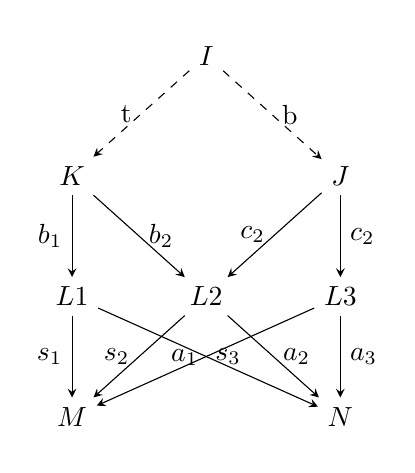
\begin{tikzpicture}
  \matrix (m) [matrix of math nodes, row sep=3em,
    column sep=3em]{
    & I & \\
    K &  & J \\
    L1 & L2 & L3 \\
    M & & N \\};
  \path[-stealth]
    (m-1-2) edge [dashed] node [left] {t} (m-2-1) 
    		edge [dashed] node [right] {b} (m-2-3)
    (m-2-1) edge node [left] {$b_1$} (m-3-1) edge node [right] {$b_2$} (m-3-2)
    (m-2-3) edge node [left] {$c_2$} (m-3-2) edge node [right] {$c_2$} (m-3-3)
    (m-3-1) edge node [left] {$s_1$} (m-4-1) edge node [left] {$a_1$} (m-4-3)
    (m-3-2) edge node [left] {$s_2$} (m-4-1) edge node [right] {$a_2$} (m-4-3)
    (m-3-3) edge node [right] {$s_3$} (m-4-1) edge node [right] {$a_3$} (m-4-3);
            \end{tikzpicture}

\

%*DIAGRAM*: by (D2) there exists a $u$ from H to I, get all paths $H \rightarrow M$ and $H \rightarrow N$ commute ( CHECK AGAIN) and all paths ending in M are in S. 

\

\begin{tikzpicture}
\matrix (m) [matrix of math nodes, row sep=3em, column sep=3em]{
& H & \\
& I & \\
K & & J \\
& L2 & \\};
\path[-stealth]
(m-1-2) edge [dashed] node [right] {u} (m-2-2)
(m-2-2) edge node [left] {t} (m-3-1) edge node [right] {b} (m-3-3)
(m-3-1) edge node [left] {$b_2$} (m-4-2)
(m-3-3) edge node [right] {$c_2$} (m-4-2);
   \end{tikzpicture}

\

So we get $(a_1, s_1) \sim (a_3,s_3)$.  With this transitivity, we have that $\sim$ is an equivalence relation.


\

So we can quotient $A\times S$ by $\sim$ to define the set $A_S$.

\

We define composition of two morphisms $q_1 \in A_S(M_0,M_1), q_2 \in A_S(M_1,M_2)$ by choosing representatives $(a_i,s_i)\in A\times S(M_{i-1},M_i)$ such that $q_i = \overline{(a_i,s_i)}$.

\

%*DIAGRAM* OF MORPHISMS; highlight $a_1, s_2$, fill box with $c, u$ from $K$

\

\begin{tikzpicture}
\matrix (m) [matrix of math nodes, row sep=3em, column sep=3em]{
& & K & & \\
& L & & L' & \\
M0 & & M1 & & M2 \\};
\path[-stealth]
(m-1-3) edge [dashed] node [left] {u} (m-2-2) 
		edge [dashed] node [right] {c} (m-2-4)
(m-2-2) edge node [left] {$s_1$} (m-3-1) 
		edge node [right] {$a_1$} (m-3-3)
(m-2-4) edge node [left] {$s_2$} (m-3-3) 
		edge node [right] {$a_2$} (m-3-5);
   \end{tikzpicture}

\

(caption) By (D1), given $a_1, s_2$ we have $c,u$ from $K$ such that $a_1 \circ c = s_2 \circ u$.

\

Let $q_2 \circ q_1 = \overline{(a_2 \circ c, s_1 \circ u)}$.  We now to check this is well-defined:

\

Suppose $q_i' = \overline{(a_i',s_i')}$ and choose $u', c'$.  We must show that $\overline{(a_2 \circ c, s_1 \circ u)} = \overline{(a_2' \circ u', s_1' \circ c')}$.  

\

Since $(a_i,s_i) \sim (a_i', s_i')$, there exist $b_i, b_i'$ from $Ji$ such that:

\

%*DIAGRAM*: two triangles up from each pair $(M_0,M_1), (M_1,M_2)$ with tops $L_i,, L_i'$, connect each triangle pair top vertex with $(b_i, b_i')$ pair $J_i$ 

\

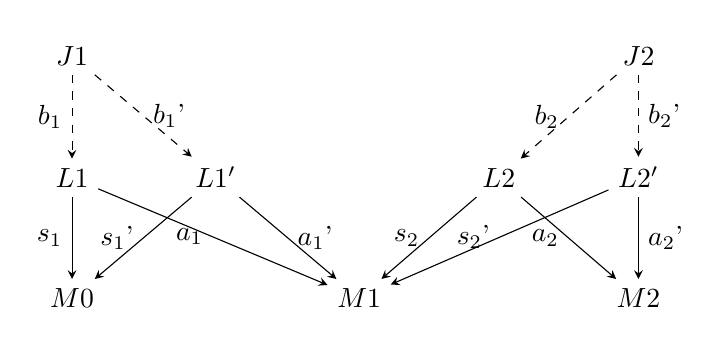
\begin{tikzpicture}
  \matrix (m) [matrix of math nodes, row sep=3em,
    column sep=3em]{
    J1 & & & & J2 \\
    L1 & L1' & & L2 & L2' \\
    M0 & & M1 & & M2 \\};
    \path[-stealth]
   (m-1-1) edge [dashed] node [left] {$b_1$} (m-2-1)
   		edge [dashed] node [right] {$b_1$'} (m-2-2)
   (m-1-5) edge [dashed] node [left] {$b_2$} (m-2-4)
   		edge [dashed] node [right] {$b_2$'} (m-2-5)
    (m-2-1) edge node [left] {$s_1$} (m-3-1)
    		edge node [ left] {$a_1$} (m-3-3)
  (m-2-2) edge node [left] {$s_1$'} (m-3-1)
  	   edge node [right] {$a_1$'} (m-3-3)
(m-2-4) edge node [left] {$s_2$} (m-3-3)
    		edge node [ left] {$a_2$} (m-3-5)
  (m-2-5) edge node [left] {$s_2$'} (m-3-3)
  	   edge node [right] {$a_2$'} (m-3-5);
\end{tikzpicture}

\

%*DIAGRAM*: include K, K' roof up between (L1,L2) and (L1',L2') by (D1);

By (D1) we get the compositions through $K, K'$ commute to $M1$ (CHECK PHRASING)

\

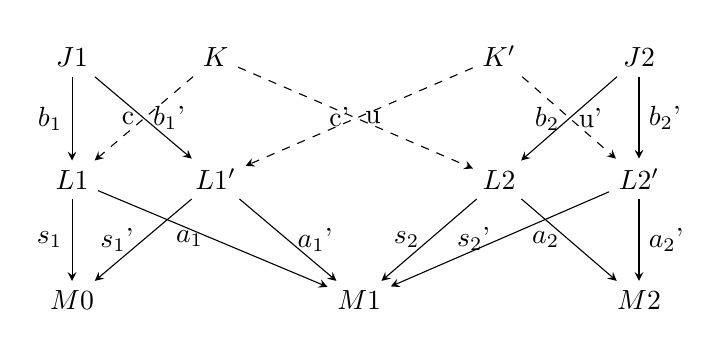
\begin{tikzpicture}
  \matrix (m) [matrix of math nodes, row sep=3em,
    column sep=3em]{
    J1 & K & & K' & J2 \\
    L1 & L1' & & L2 & L2' \\
    M0 & & M1 & & M2 \\};
    \path[-stealth]
   (m-1-1) edge node [left] {$b_1$} (m-2-1)
   		edge  node [right] {$b_1$'} (m-2-2)
   (m-1-5) edge node [left] {$b_2$} (m-2-4)
   		edge node [right] {$b_2$'} (m-2-5)
    (m-2-1) edge node [left] {$s_1$} (m-3-1)
    		edge node [ left] {$a_1$} (m-3-3)
  (m-2-2) edge node [left] {$s_1$'} (m-3-1)
  	   edge node [right] {$a_1$'} (m-3-3)
(m-2-4) edge node [left] {$s_2$} (m-3-3)
    		edge node [ left] {$a_2$} (m-3-5)
  (m-2-5) edge node [left] {$s_2$'} (m-3-3)
  	   edge node [right] {$a_2$'} (m-3-5)
(m-1-2) edge [dashed] node [left] {c} (m-2-1)
	edge [dashed] node [right] {u} (m-2-4)
(m-1-4) edge [dashed] node [left] {c'} (m-2-2)
	edge [dashed] node [right] {u'} (m-2-5);	   
\end{tikzpicture}

\

%*DIAGRAM*:  include $I_1$ between $J_1$ and $K$ by (D1), include $\tilde{I_2}$ roof between K' and J2 by (D1),

By (D1) again, we get the diagram commutes above $L1$ and through $L2'$ to $M1$

\

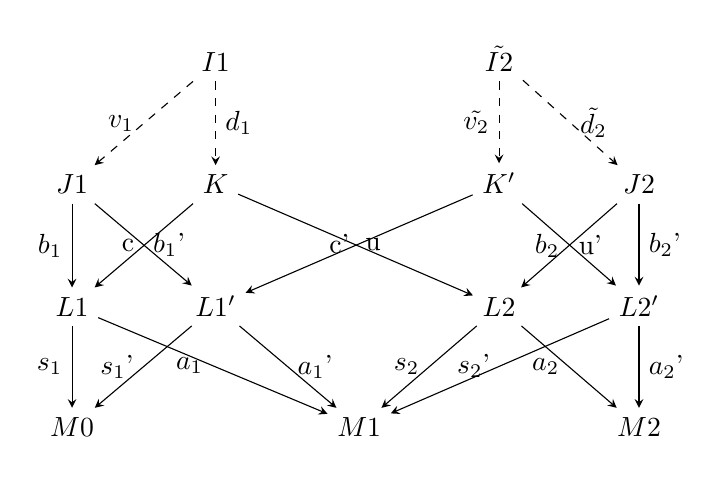
\begin{tikzpicture}
  \matrix (m) [matrix of math nodes, row sep=3em,
    column sep=3em]{
    & I1 & & \tilde{I2} &\\
    J1 & K & & K' & J2 \\
    L1 & L1' & & L2 & L2' \\
    M0 & & M1 & & M2 \\};
    \path[-stealth]
    (m-1-2) edge [dashed] node [left] {$v_1$} (m-2-1)
    		edge [dashed] node [right] {$d_1$} (m-2-2)
 (m-1-4) edge [dashed] node [left] {$\tilde{v_2}$} (m-2-4)
 		edge [dashed] node [right] {$\tilde{d_2}$} (m-2-5)
   (m-2-1) edge node [left] {$b_1$} (m-3-1)
   		edge  node [right] {$b_1$'} (m-3-2)
   (m-2-5) edge node [left] {$b_2$} (m-3-4)
   		edge node [right] {$b_2$'} (m-3-5)
    (m-3-1) edge node [left] {$s_1$} (m-4-1)
    		edge node [ left] {$a_1$} (m-4-3)
  (m-3-2) edge node [left] {$s_1$'} (m-4-1)
  	   edge node [right] {$a_1$'} (m-4-3)
(m-3-4) edge node [left] {$s_2$} (m-4-3)
    		edge node [ left] {$a_2$} (m-4-5)
  (m-3-5) edge node [left] {$s_2$'} (m-4-3)
  	   edge node [right] {$a_2$'} (m-4-5)
(m-2-2) edge node [left] {c} (m-3-1)
	edge  node [right] {u} (m-3-4)
(m-2-4) edge node [left] {c'} (m-3-2)
	edge node [right] {u'} (m-3-5);	   
\end{tikzpicture}

\

%*DIAGRAM *by (D2) there is a $\tilde{v} \in S$ such that $I2 \xrightarrow{\tilde{v}} \tilde{I2}$ and paths $I2 \rightarrow L2'$ are equal

By (D2), we get commutation above $L2'$

\

\begin{tikzpicture}
  \matrix (m) [matrix of math nodes, row sep=3em,
    column sep=3em]{
 & I2 & \\
 & \tilde{I2} & \\
 K' & & J2 \\
 & L2' & \\
 & M1 & \\};
    \path[-stealth]
(m-1-2) edge [dashed] node [left] {$\tilde{v	}$} (m-2-2)
(m-2-2) edge node [left] {$\tilde{v_2}$} (m-3-1)
	 edge node [right] {$\tilde{d_2}$} (m-3-3)
(m-3-1) edge node [left] {c'} (m-4-2)
(m-3-3) edge node [right] {$b_2$'} (m-4-2)
(m-4-2) edge node [left] {$s_2$'} (m-5-2);   
\end{tikzpicture}


\

At this point, we've constructed the following diagram so that is is all commutative.

\

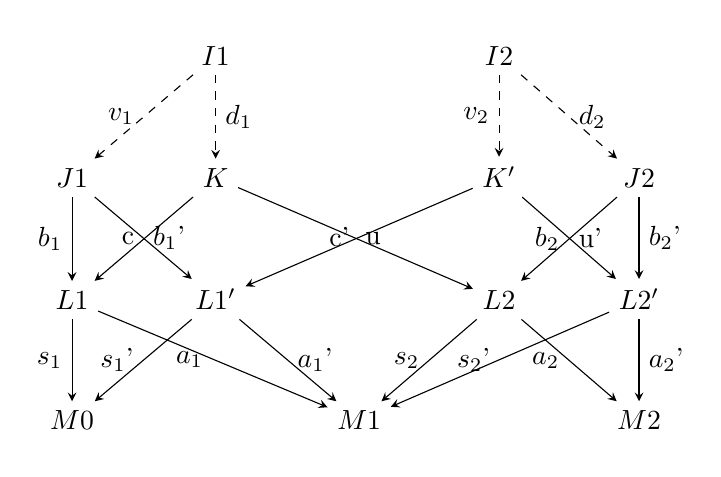
\begin{tikzpicture}
  \matrix (m) [matrix of math nodes, row sep=3em,
    column sep=3em]{
    & I1 & & I2 &\\
    J1 & K & & K' & J2 \\
    L1 & L1' & & L2 & L2' \\
    M0 & & M1 & & M2 \\};
    \path[-stealth]
    (m-1-2) edge [dashed] node [left] {$v_1$} (m-2-1)
    		edge [dashed] node [right] {$d_1$} (m-2-2)
 (m-1-4) edge [dashed] node [left] {$v_2$} (m-2-4)
 		edge [dashed] node [right] {$d_2$} (m-2-5)
   (m-2-1) edge node [left] {$b_1$} (m-3-1)
   		edge  node [right] {$b_1$'} (m-3-2)
   (m-2-5) edge node [left] {$b_2$} (m-3-4)
   		edge node [right] {$b_2$'} (m-3-5)
    (m-3-1) edge node [left] {$s_1$} (m-4-1)
    		edge node [ left] {$a_1$} (m-4-3)
  (m-3-2) edge node [left] {$s_1$'} (m-4-1)
  	   edge node [right] {$a_1$'} (m-4-3)
(m-3-4) edge node [left] {$s_2$} (m-4-3)
    		edge node [ left] {$a_2$} (m-4-5)
  (m-3-5) edge node [left] {$s_2$'} (m-4-3)
  	   edge node [right] {$a_2$'} (m-4-5)
(m-2-2) edge node [left] {c} (m-3-1)
	edge  node [right] {u} (m-3-4)
(m-2-4) edge node [left] {c'} (m-3-2)
	edge node [right] {u'} (m-3-5);	   
\end{tikzpicture}

\

% *DIAGRAM* by (D1) choose $w \in A$ and $e \in S $from H to fill in $I_1 \rightarrow M_0 \leftarrow I_2$;

By (D1), we can get commutation into $M0$ from $I1$ and $I2$ by considering $w \in A$ and $e \in S$ from $H$.  

\

INSERT DIAGRAM H THROUGH MS


\

While $H \rightarrow I_2 \rightarrow M_0 \in S$, we could fail to have commuting paths $H \rightarrow L_1'$ and $H \rightarrow L2$.

\

\begin{tikzpicture}
  \matrix (m) [matrix of math nodes, row sep=3em,
    column sep=3em]{
 & & H & & \\
 & I1 & & I2 & \\
 J1 & K & & K' & J2\\
 & L1' & & L2 &\\};
    \path[-stealth]
(m-1-3) edge [dashed] node [left] {w} (m-2-2)
	edge [dashed] node [right] {e} (m-2-4)
(m-2-2) edge node [left] {$v_1$} (m-3-1)
	edge node [right] {$d_1$} (m-3-2)
(m-2-4) edge node [left] {$v_2$} (m-3-4)
	edge node [right] {$d_2$} (m-3-5)
(m-3-1) edge node [left] {$b_1$'} (m-4-2) 
(m-3-2) edge node [left] {c} (m-4-4)
(m-3-4) edge node [right] {u'} (m-4-2)
(m-3-5) edge node [right] {$b_2$} (m-4-4);
\end{tikzpicture}

\

% INCLUDE SAME DIAGRAM, with highlighting: NOTE, $H \rightarrow I_2 \rightarrow M_0 \in S$ but could fail to commute in paths $H \rightarrow L_1'$ and $H \rightarrow L2$.

\

Noting that upon composing with $s_1'$ into $M0$, our paths from $H \rightarrow L_1'$ become equal, so by (D2) we get $w' \in S$ from $H'$ such that we now have commutation above $L_1'$.


\

For the same reasons with composition with $s_2$, we get commutation above $L_2$ when mapping from $H''$. (CHECK, DOESN'T MAKE SENSE B/C DON'T HAVE COMMUTATION ABOVE $M1$ YET, DO WE?)


\

Now all paths $H'' \rightarrow M_2$ are equal and all paths $H'' \rightarrow M0$ are equal and in S.

\

INCLUDE FINAL DIAGRAM: i.e. $(a_2 \circ c, s_1 \circ u) \sim (a_i' \circ c', s_1' \circ u')$.

\

We are done with proving well-defined composition.  Take the identity morphism to be $\overline{(1_M,1_M)}$.

\

One now must check the identity and associativity properties of this definition of composition.  

\

Define $Q: A \rightarrow A_s$ to be $Q(M) = M, Q(a) = \overline{(a,1_M)}$ for $a: M \rightarrow N$.  One must also chech that $Q$ is indeed a functor.

\

We now verify that the axioms of right Ore localization are satisfied.  We have (L1) satisfied by our definition of Q.  We can easily check that the inverse of Q(s) is $\overline{(1,s)}$ to get (L2) and $\overline{(a,s)} = \overline{(a,1)}\circ \overline{(1,s)}$ to get (L3).  Lastly, we have $Q(a_1)  = Q(a_2)$ means that $(a_1, 1) \sim (a_2, 1)$, so there exist $b_1, b_2 \in A$ such that $a_1 \circ b_1 = a_2 \circ b_2$ and $1 \circ b_1 = 1 \circ b_2 \in S$.  Let $s = b_1 \in S$, get $a_1 \circ S = a_2 \circ S$.


\end{proof}

\

\section{Cohomological Functors Revisited, briefly}


\

KEY Prop (11.2.1?): If H: K $\rightarrow $M is a cohomological functor from a triangulated category K to an abelian category M and we consider $S = \{ s \in K | H(T^i(s)) $ is invertible for all $i \in \mathbb{Z}\}$.  Then $S$ is a left and right denominator set.  

\

\section{Localization of Triangulated categories:}

%SEEMS LIKE TIME FOR PROOFS, TIEING THINGS TOGETHER TO GET DERIVED CATEGORY WITH TRIANGULATED STRUCTURE. 

\

KEY Thm (11.2.2) If $S$ is the right denominator set associated to a cohomological functor on $K$, and $(K_S, Q)$ is the right Ore localization, then $K_S$ has a unique triangulated structure such that (i) Q is a triangulated functor (ii) if $F : K \rightarrow E$ is another triangulated functor such that $F(s)$ is invertible for all $s \in S$, then the localization $F_S: K_S \rightarrow E$ is triangulated.

\

\section{The Big Reveal...}

STATE DEF OF DERIVED CATEGORY IN TERMS WE"VE JUST BUILT UP.  MAYBE STILL NEED TO SHOW $H^0$ IS COHOMOLOGICAL FUNCTOR.

\end{document}
